\documentclass[border =3mm]{standalone}
\usepackage{tikz}
\usetikzlibrary{positioning, calc, decorations.markings}

\tikzset{
    mid arrow/.style={postaction={decorate,decoration={markings,mark=at position #1 with {\arrow{stealth}}}}},
    connect/.style={mid arrow=#1, out=0, in=180, ->, >=stealth, looseness=2},
    connect/.default=6mm
}
\begin{document}

    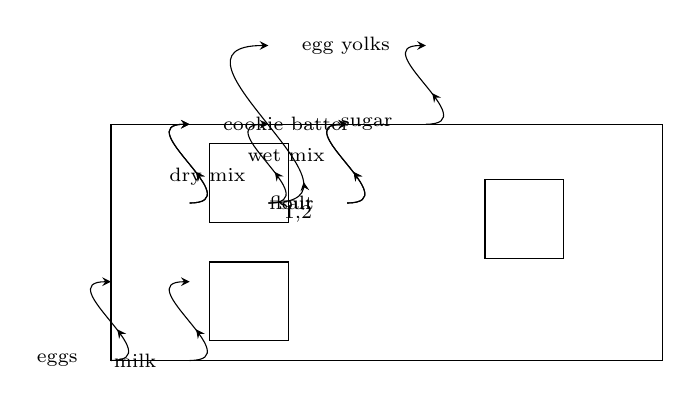
\begin{tikzpicture}
        \coordinate (SW) at (0,0); \coordinate (SE) at (7,0);
        \coordinate (NE) at (7,3); \coordinate (NW) at (0,3);
        %Frames
        \draw[black] (SW) rectangle (NE);
        \node[draw, minimum size=1cm] (dry) at ({$(NW)!0.25!(NE)$} |- {$(SW)!0.75!(NW)$}) {};
        \node[draw, minimum size=1cm] (wet) at ({$(NW)!0.25!(NE)$} |- {$(SW)!0.25!(NW)$}) {};
        \node[draw, minimum size=1cm] (mix) at ({$(NW)!0.75!(NE)$} |- {$(SW)!0.6!(NW)$}) {};
        %Extra coordinates for path
        \pgfmathsetmacro{\dx}{3}
        \foreach \y [evaluate=\y as \dy using \y/6] in {1,...,5}{
            \coordinate (W\y) at ([xshift=-\dx mm]$(SW)!\dy!(NW)$);
        }
        \foreach \y [evaluate=\y as \dy using \y/4] in {1,...,3}{
            \coordinate (dryW\y) at ([xshift=\dx mm]$(dry.south west)!\dy!(dry.north west)$);
        }
        \foreach \y [evaluate=\y as \dy using \y/2] in {1}{
            \coordinate (dryE\y) at ([xshift=-\dx mm]$(dry.south east)!\dy!(dry.north east)$);
        }
        \foreach \y [evaluate=\y as \dy using \y/3] in {1,2}{
            \coordinate (wetW\y) at ([xshift=\dx mm]$(wet.south west)!\dy!(wet.north west)$);
        }
        \foreach \y [evaluate=\y as \dy using \y/3] in {1,2}{
            \coordinate (wetE\y) at ([xshift=-\dx mm]$(wet.south east)!\dy!(wet.north east)$);
        }
        \foreach \y [evaluate=\y as \dy using \y/3] in {1,2}{
            \coordinate (mixW\y) at ([xshift=\dx mm]$(mix.south west)!\dy!(mix.north west)$);
        }
        \foreach \y [evaluate=\y as \dy using \y/2] in {1}{
            \coordinate (mixE\y) at ([xshift=-\dx mm]$(mix.south east)!\dy!(mix.north east)$);
        }
        \foreach \y [evaluate=\y as \dy using \y/3] in {1,2}{
            \coordinate (E\y) at ([xshift=\dx mm]$(SE)!\dy!(NE)$);
        }
        %Paths (left-right, bottom-up)
        \path[every node/.style={font=\scriptsize}]
            (0,0) edge[connect] node[pos=0.0, left=3mm] {eggs} (0,1)
            (1,0) edge[connect] node[pos=0.0, left=3mm] {milk} (1,1)
            (3,2) edge[connect] node[pos=0.0, left=3mm] {salt} (3,3)
            (4,3) edge[connect] node[pos=0.0, left=3mm] {sugar} (4,4)
            (3,2) edge[connect] node[pos=0.0, left=3mm] {flour} (3,3)
            (2,2) edge[connect] node[pos=0.12, below] {1,2} node[pos=1.0, right=3mm] {egg yolks}(2,4)
            (2,2) edge[connect] node[pos=0.2, above=3mm] {wet mix} (2,3)
            (1,2) edge[connect] node[pos=0.2, above] {dry mix}(1,3)
            (1,2) edge[connect] node[pos=1.0, right=3mm] {cookie batter}(1,3);
    \end{tikzpicture}

\end{document}